\documentclass[main]{subfiles}


\begin{document}
\newpage
\section{Learning Rules}

Learning rules, as the name imply, describe methods of learning from information. Various machine learning methods that we discuss elsewhere already describe ways in which the data available to us can be used to create an objective (or cost, or loss) function which gives us something concrete to optimize so we have a model that performs well on similar data. These methods describe \textbf{global} cost functions because these expressions are in terms of high-level representations in the model, often only the final output layer representations. In a very small toy model, such as a fully-connected neural network with no hidden layers, this may provide useful information for adapting individual neuronal connections. Expanding this model to add complexities such as additional neurons hidden layers leaves us with an architecture that we can understand and can enumerate, as well as the global objective which we continue to aim for. However, we now have little understanding of how individual connections should be modified in the training process to contribute to improving the global objective defined by some global cost function which makes claims describing how output representations should change to improve the model but no inherent claims describing how the changes can be implemented.

To this end, the local learning rules we are about to discuss can alternatively be considered \textbf{local optimization principles}, as they are a small instance (typically involving only a few neurons) of our global optimization goal.

\subsection{Error minimization rules}
The first category of learning rules we will discuss are those that focus on optimizing with respect to some error function.

\subsubsection{Perceptron learning rule}

The perceptron learning rule was inspired by the model of neurons at the time, chiefly outlined in the McCulloch and Pitts Neuron. This model describes basic action potential propagation and involves multiple presynaptic neurons connected to the soma of a postsynaptic neuron. An action potential is triggered when sufficiently many presynaptic neurons (which may each contribute differently to the postsynaptic neuron based on their synaptic strengths) are activated such that the joint effects of their action potentials in the postsynaptic neuron exceeds the activation threshold, which triggers an action potential through the postsynaptic neuron.

Analogously, the perceptron learning rule involves multiple input values, which are each connected with varying weights to an output node. The value emitted by the output node depends on whether the weighted contributions of the input values exceeds a specific threshold. Learning is the process of adjusting the weights of each input as well as the output threshold to achieve the desired goal.

This can be denoted by a thresholded linear transformation. Given an input vector of values, the output falls into two cases depending on whether the linear transformation is above or below the threshold. Specifically, for an input vector $x$, corresponding weights $w$, and a threshold $b$, the output can be denoted as:
\begin{equation}
    \text{output} =
    \begin{cases}
      0, & \text{if}\ w \cdot x + b \leq 0 \\
      1, & \text{if}\ w \cdot x + b > 0
    \end{cases}
  \end{equation}

As a result, from a machine learning classification perspective, the perceptron learning rule describes a linear classifier as its decision is based on the result of a linear transformation. The standard algorithm (developed by Rosenblatt) for training according to this learning rule involves looping through every data sample, updating the weights $w$ if and only if the current data sample $x$ is misclassified, detailed below:
\begin{figure}[H]
		\centering
		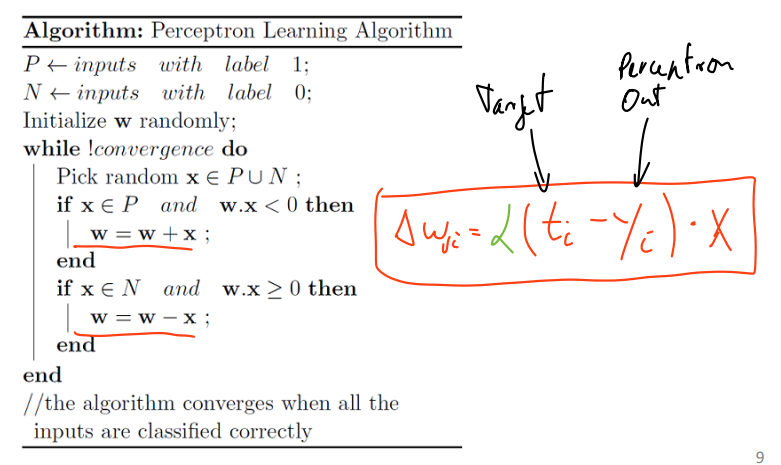
\includegraphics[width=0.8\linewidth]{04_LearningRules/figures/4_1_perceptron.png}
		\caption{Algorithm for the perceptron learning rule}
		\label{fig:4_perceptron}
	\end{figure}

As shown in Figure \ref{fig:4_perceptron}, if $x$ is a false positive, the new $w$ is the sum of the current $w$ and $x$. If $x$ is a false negative, the new $w$ is the difference between the current $w$ and $x$. The algorithm concludes when all samples are classified correctly, i.e. $w$ does not change after looping through all samples. If the points are not linearly separable (there exists no linear decision boundary that discriminates positive and negative samples) the algorithm will oscillate and the weights $w$ will fail to converge.

\subsubsection{ADALINE learning rule}

This can be viewed as a slightly modified instance of the perceptron learning rule. In the perceptron rule, the thresholded result of the weighted sum of inputs is used for updating the weights in each iteration. In ADALINE, the weighted sum of inputs ($w \cdot x$ above) itself is used to update the weights in training.

\subsubsection{DELTA learning rule}

The weight updates from this equation aim to directly minimize a neuron's output error for a target value $t_i$ and output value $y_i$, which can be formulated using gradient descent minimizing the squared error between these values.

This error can be formulated as:
$$E = \frac{1}{2} (t_i - y_i)^2$$

Finding the appropriate weight updates according to the gradient descent optimization method requires calculating the change in error with respect to each weight that we wish to update. This can be expressed as:
$$\frac{\partial E}{\partial w_{ji}} = \frac{\partial \frac{1}{2} (t_i - y_i)^2}{\partial w_{ji}}$$

Assuming a model structured similarly as in the perceptron and ADALINE learning rules with a single layer between inputs and the output value, this yields:

$$\nabla w_{ji} = \alpha (t_i - y_i) g^'(h_i) x_i$$

for some learning rate $\alpha$, target value $t_i$ and output $y_i$, derivative $g'$ of the activation function $g$, sum of inputs $h_i$, and input $x_i$.

The weight update equation for the DELTA learning rule clearly shares some similarities with that of the perceptron learning rule. Both weight update equations contain an error term calculated by the difference between the target and output values $(t_i - y_i)$ multiplied with the input $x_i$. However, the DELTA learning rule adds some complexities as it incorporates a learning rate $\alpha$ to adapt learning as well as the derivative of the activation function applied to the sum of the inputs $g'(h_j)$.

While the perceptron learning rule, particularly in light of its well-defined algorithm, defines the problem in terms of shifting hyperplanes to adapt a decision boundary, the DELTA learning rule optimizes the sum of squared error for a model with an activation function applied to a linear output. As previously mentioned in the contrast between the perceptron and ADALINE rules, the perceptron rule will either reach a stable zero-error solution (in the case of linearly separable data) or continually oscillate (otherwise). In contrast, the DELTA rule due in part to its adaptable learning rate can continually converge to a minimum error solution.

\subsection{Biologically plausible rules}
\subsubsection{Hebbian learning}
\epigraph{Cells that fire together wire together.}{Not a direct quote by Hebb}

\begin{figure}[H]
		\centering
		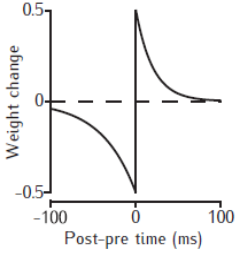
\includegraphics[width=0.4\linewidth]{04_LearningRules/figures/4_2_hebbian.png}
		\caption{A schematic of theoretical pre- and postsynaptic spike timing correlation with weight updates: LTP ($>0$ ms) or LTD ($<0$ ms)}
		\label{fig:4_hebbian}
	\end{figure}

Spike-timing dependent plasticity is the Hebbian learning concept of weights between neuronal synapses changing over time based on the timing of their spikes. If a postsynaptic neuron fires at the same time or just after the presynaptic neuron fires, whether this is due to an action potential in the presynaptic neuron or other nearby neurons, this indicates that connections between these two neurons could be reinforced, which occurs by increasing the weights on these synaptic junctions to more efficiently propagate future action potentials. This is known as long-term potentiation. However, if a postsynaptic neuron fires just before a presynaptic neuron, the junction in the pre- to postsynaptic direction is possibly unnecessary or counterproductive so the weight of these synapses decrease over time. This is known as long-term depression.

We can start by writing a simple Hebbian weight update as the product of the input and output with some scaling factor:
\begin{align}
     w &= \alpha \times x \times y\\
        &= \alpha \times x \times [w \cdot x]\\
\end{align}

The more closely aligned $w$ and $x$ are, the larger $y = w^T x$ is, and by definition of the dot product $y = 0$ when $w$ is orthogonal to $x$. This leads to the weight vector gradually pointing towards the input vector, or the cloud of input data in a dataset. We can mitigate this issue by applying a zero-mean transformation on our dataset to center the data around the origin, but this leads to a different problem of the weight vector tending to align with the direction of greatest variance.

Let's explore some other ways to express this Hebbian update rule:
\begin{align}
    \nabla w &= \alpha \times x \times y\\
        &= \alpha (w \cdot x) x\\
        &= \alpha (x \cdot x^T) \cdot w
\end{align}
where the last step involves a transformation of the inner product into an outer product, which was skipped in lecture but is detailed in a dedicated lecture slide.

We note that $x \cdot x^T$ is the correlation matrix of the vector $x$, which we denote as $C$. \textit{This is distinct from the covariance matrix.} We now arrive at:
\begin{align}
    \nabla w &= \alpha (x \cdot x^T) \cdot w\\
        &= \alpha \times C \cdot w\\
    \text{which leads to the following update over time:}\\
    \frac{\partial w}{\partial t} &= C \cdot w
\end{align}

The lecture slides go into some more detail describing that applying the classical solution for this expression, $w(t) = u \times e^{\lambda \times t}$ for some vector $u$, as $\lambda$ is positive the weight vectors will continue to increase and blow up.

\subsubsection{Oja's rule}

A modification of the Hebbian rule above in which a weight decay term is added. As this weight decay term is proportional to $y^2$, a quadratic result, it eventually limits the magnitude of the weights $w$ to unit length while maintaining the tendency of the weights to point in the direction of maximum variance.
\begin{align}
    \nabla w_{oja} = \nabla w - y^2 \times w &= \alpha \times x \times y - y^2 \times w\\
        &= \alpha \times y (x - y \times w)
\end{align}

\subsubsection{Covariance rule}

Another modification of the Hebbian rule above uses an idea similar to mean-centering of the data, but instead of transforming the data, the weights $w$ are updated using mean-centered inputs $x$ and outputs $y$.
\\ \\
Notation: $\langle \cdot \rangle$ denotes the mean of the variable over the input samples.

\begin{align}
    \nabla w_{cov} &= \alpha \big[y - \langle y\rangle\big]\big[x - \langle x\rangle\big]\\
        &= \alpha \big[y \times x - \langle y\rangle \times x - y \times \langle x\rangle + \langle y\rangle \times \langle x\rangle\big]
\end{align}
\begin{align}
    \langle \nabla w_{cov}\rangle &= \alpha \big[\langle y \times x\rangle - \langle \langle y\rangle \times x\rangle - \langle y \times \langle x\rangle\rangle + \langle \langle y\rangle \times \langle x\rangle\rangle\big]\\
    &= \alpha \big[\langle y \times x\rangle - \langle y\rangle \times \langle x\rangle - \langle y\rangle \times \langle x\rangle + \langle y\rangle \times \langle x\rangle\big]\\
    &= \alpha \big[\langle y \times x\rangle - \langle y\rangle \times \langle x\rangle\big]
\end{align}

The last line depicts the difference between the mean of the product of $x$ and $y$, $\langle y \times x\rangle$ and the product of the means $\langle y\rangle \times \langle x\rangle$.

This rule solves a similar problem as Oja's rule, specifically the blowing up of weights over the training process. By subtracting the means when updating, weight updates can be negative as well as positive. The weights $w$ increase when pre- and post-synaptic firing are positively correlated, and the change is proportional to the covariance of the firing rates.

\subsubsection{Sanger's rule}

The idea is that we use a single Hebbian neuron that points in the direction of maximum variance, as described previously, and view this as a principal component of the data. We subtract the contribution of this first principal component from the data, feeding the remaining data into a different neuron which subsequently identifies the direction of maximum variance in this data. This process can be repeated and resembles the addition of principal components in Principal Component Analysis (PCA).

\subsubsection{Sejnowski's Infomax rule}

The Infomax rule utilizes a nonlinear function and yields a method for implementing Independent Component Analysis (ICA).

\subsubsection{Bienenstock-Cooper-Monroe rule}

\begin{figure}[H]
		\centering
		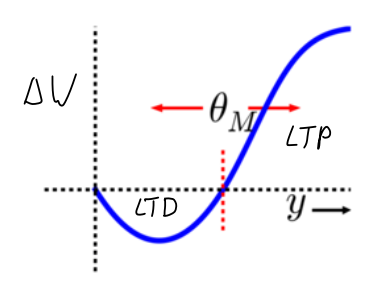
\includegraphics[width=0.5\linewidth]{04_LearningRules/figures/4_3_bcm.png}
		\caption{BCM rule}
		\label{fig:4_bcm}
	\end{figure}

Activity is measured by $y$ along the horizontal axis, and with no activity no change in weights takes place. Activity below a certain threshold $\theta_M$ triggers the LTD regime, and activity above this threshold triggers the LTP regime.

Measuring neuronal output across a certain window indicates that there is a biological basis for this. Above some threshold, the weight updates increased as the stimulation frequency was increased.

This was tested experimentally in the hippocampus and primary visual cortex, stimulating inputs to a neuron and measuring its spiking frequency. In this experiment, below a stimulation frequency of about 10 Hz the weight updates were negative, while above this stimulation frequency they were positive.

\subsubsection{Triplet rule}

\begin{figure}[H]
		\centering
		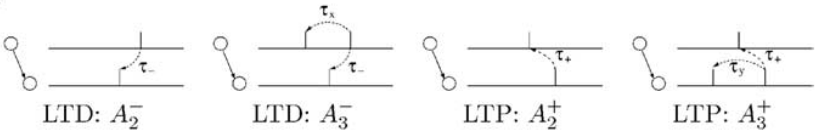
\includegraphics[width=\linewidth]{04_LearningRules/figures/4_4_triplet.png}
		\caption{Examples of pre- (top) and postsynaptic (bottom) spike pairs and triplets leading to LTD or LTP}
		\label{fig:4_triplet}
	\end{figure}

The triplet rule extends the classical Hebbian STDP idea. Instead of only looking at single presynaptic and postsynaptic spikes, multiple recent spikes within a specified time window are considered. As shown in Figure \ref{fig:4_triplet}, LTD generally occurs when a presynaptic spike occurs just after a postsynaptic spike, even if (as in $A^-_3$) another presynaptic spike preceded the postsynaptic spike. Analogously, LTP tends to occur when a postsynaptic spike follows a presynaptic spike, even if (as in $A^+_3$) another postsynaptic spike preceded the presynaptic spike. In this fashion, the consideration of the third spikes within the time window can lead to different outcomes.

In both the triplet and BCM rules, above some threshold as the spiking frequency increases, the weight updates also increase (and are positive).

The fundamental differences between these two rules are unclear.

\subsubsection{Calcium rule}

As shown in Figure \ref{fig:4_calcium}, this rule specifies that the LTP regime applies based on the amount of time above the calcium threshold while the LTD regime applies below the threshold. This rule results in the same basic STDP profile as before, and there are threshold parameters that can be changed to affect the dynamics.

\begin{figure}[H]
		\centering
		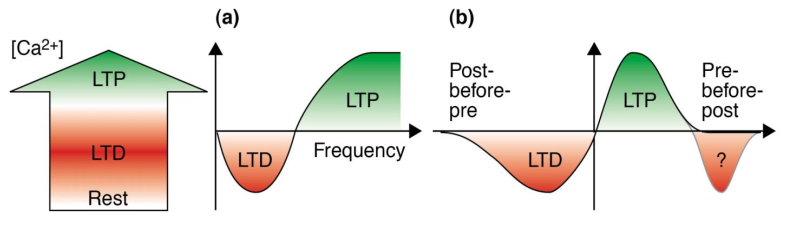
\includegraphics[width=0.8\linewidth]{04_LearningRules/figures/4_5_calcium.png}
		\caption{Calcium rule}
		\label{fig:4_calcium}
	\end{figure}

\subsubsection{Hebbian learning: Unsupervised}

Error-driven learning appears to be much more necessary for deeper networks. A network was trained on the MNIST dataset (handwritten digits) using a basic Hebbian learning rule to cluster the data into separate digits and then learn a linear classifier on these digits.

\subsubsection{Hebbian learning: Three-factor rules}

\begin{figure}[H]
		\centering
		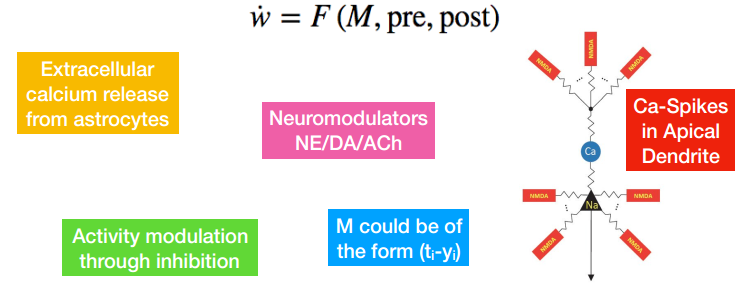
\includegraphics[width=1.0\linewidth]{04_LearningRules/figures/4_6_three-factor.png}
		\caption{Possible third factors $M$ in three-factor learning rules}
		\label{fig:4_threefactor}
	\end{figure}

Three-factor Hebbian learning rules integrate the pre- and postsynaptic firing with a third factor, $M$, which includes values such as the covariance-rule, TD learning, gated Hebbian learning, surprise-modulated STDP, etc.

For a biological neuron, this $M$ factor may be viewed in a variety of ways, as shown in Figure \ref{fig:4_threefactor}.

It may be seen as a representation of error, including backpropagated error. For example, in the apical dendrites (level 5 neurons) receive feedback signals from the next hierarchical layer, and the strong calcium channels in these apical dendrites allow for error signals to trigger calcium spikes that propagate down the cell. The calcium spike is therefore a possible representation of the error from the next layer, which would model backpropagation.

Alternatively, neurons project to the next layer but some also project backwards to interneurons (and in turn, back to the apical dendritic layer), so the error signals reflect what is happening globally, in the next layer, and (through lateral inhibition, etc.) what is occurring in neighboring neurons. There is a motivation, as seen in the learning rules that are analogous to PCA, to inhibit neighboring neurons. In particular, this allows a neuron to potentially learn a useful unique representation instead of learning the same things as every other neuron.

Another possibility includes extracellular calcium release from astrocytes, as this affects the external calcium concentration but also internal concentrations in neurons, thereby indirectly affecting the plasticity of said neuron.

\end{document}